\subsection{Installing an APK} \label{subsection:android-install}
Before running an application, its \gls{apk} has to be installed.
The installation consists of two major steps.
The first step is primarily about verification, while the second step is the bytecode optimization and, in case of \gls{art}, the code compilation (see figure~\ref{fig:install}).
The differences will be explained in the following subsections.
\newline
Before initiating the installation, the \gls{apk} is checked for a legitimate checksum, the signature is checked and the classes.dex structure is validated.
In case one action fails to validate, the installation is rejected by the OS.
\newline
The installation can be performed in two ways depending on the runtime of the Android \gls{os}.
In case the \gls{dvm}, optimisation is applied to the classes.dex file and the corresponding \gls{odex} file is generated and moved to the Dalvik cache.
As a reminder, the \gls{odex} is an optimization tailored to the specific architecture of the device in order to achieve the best performance.
This is useful due to the the high diversity of Android running hardware and their different processors.
This is done once on installation.
Future application starts will execute the \gls{odex} file instead of the the \gls{dex} file.
This preprocessed version of the application has an improved startup time. \cite{kovachevaMaster}
\newline
Currently, the Android runtime of choice is \gls{art}.
For this runtime, the second step is more complex since the bytecode has to be compiled an additional time.
This will be explained closer in section~\ref{subsection:android-art}.
\newline
After the bytecode is optimized respectively compiled, the application can be run.
\newline
\begin{figure}[h]
    \centering
    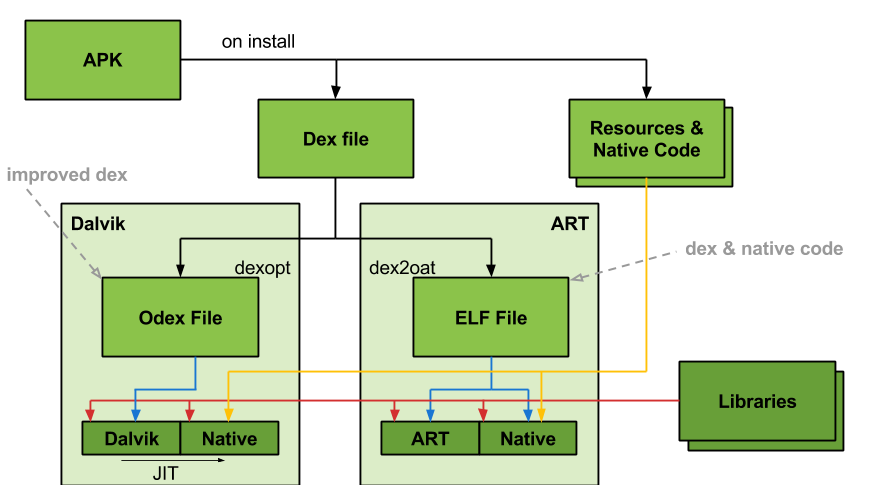
\includegraphics[width=0.8\textwidth]{data/install.png}
    \caption{Installing an \gls{apk} on a device \cite{googleIOArt}}
    \label{fig:install}
\end{figure}
When the application is run on the device, Android creates an sandboxed environment for application only.
This is achieved by assigning each process an own \gls{vm} and seperate user ID.
This way each application runs separated from the others and has no access on resources except its own. \cite{developerFundamentals}
